\begin{quote}
  Parkosz's treatise, the Unicode standard and the Junicode font
  
  Jakub Parkosz, known also as Parkoszowic, is the author of the first
  proposal of Polish spelling. To account for all the phonemes of
  Polish some new letters were proposed. As his proposal did not catch
  on, the letters haven't became available in the standard fonts,
  which made difficult to quote and discuss the proposal. Fortunately
  recently the letters has been added to the Junicode font by its
  creator Peter Baker.

  Keywords: Jakub Parkosz, hisory of Polish language, spelling,
  Unicode, Junicode
\end{quote}

\section{Parkosz}
\label{sec:parkosz}

\subsection{Traktat Parkosza}
\label{sec:traktat-parkosza}

Jakub Parkosz, inaczej Parkoszowic, jest --- jak wiadomo --- autorem
pierwszej propozycji pisowni polskiej [\cite{TraktatPWN1985}]. Skany
traktatu są dostępne m.in. pod adresem
\url{https://jsbien.github.io/Parkosz4IIIF/}. Wprowadzone przez
Parkosza --- w łacińskim rękopiśmiennym traktacie --- litery się nie
przyjęły, co od lat stwarzało problemy przy omawianiu tego traktatu
oraz wydawaniu go drukiem ---
por. \autocite{janusz_s._bien_parkoszs_2022} i
\autocite{bień22:_parkosT}.

\subsection{Cytowanie przez Stanisława Zaborowskiego}
\label{sec:cytow-przez-stan}



W traktacie Stanisława Zaborowskiego --- drugiej z kolei propozycji
pisowni polskiej --- pisownia Parkosza jest wspominana, ale w
zależności od edycji ma to różne formy, być może ze względu na inne
możliwości drukarni.

Zaborowski wspomina w szczególności o dwóch literach wprowadzonych
przez Parkosza, mianowicie \textit{b kanciastym} (inspiracją dla
Parkosza był znak muzyczny \textit{b durum}, który wówczas miał nieco
inny kształt,
% którego oryginalny
% kształt możemy zobaczyć obecnie np. w
% \autocite[s. 5]{apel69:_harvar_diction_music})
i \textit{b
okrągłym}.
% --- por. il. \vref{fig:ParkoszB} (z artykułu
% \autocite[s. 42]{bien_parkoszPSP}).


W pierwszym niedatowanym wydaniu Unglera (ok. 1513
r.)\footnote{\url{http://mbc.malopolska.pl/publication/89609}} litery
te są tylko omówione, patrz il. %\vref{fig:b-durummolleA04}. nie działało!!!
\vref{fig:b-durummolleA04problen}.

\begin{figure}[h]
    \centering
    \includegraphics[height=06ex]{img/00-a_b-durummolleA04}
    \includegraphics[height=06ex]{img/00-b_b-durummolleA04}
    \caption{Ungler ok. 1513}
    \label{fig:b-durummolleA04problen}
  \end{figure}


  W wydaniu Hallera z 1518 r.\footnote{\url{https://polona.pl/item/5158973}} \textit{b durum}
  jest zilustrowane innym znakiem muzycznym o tej samej genezie ---
  patrz il. \vref{fig:b-durummolleB03}.
  % i il. \vref{fig:PT4pismo11}.
  Jest to znak używany do dzisiaj jako tzw. kasownik.
  % , w standardzie
  % Unicode \ucode{266E} \uname{MUSIC NATURAL SIGN}.
  Litera \textit{b molle} jest
  tylko wspomniana.
  % Został on
  % uwzględniony w \textit{Polonia Typographica} w zestawie znaków pisma
  % nr 11 (\vref{fig:PT4pismo11})

    \begin{figure}[h]
    \centering
    \includegraphics[height=06ex]{img/00_b-durummolleB03}
    \caption{Haller 1518: znak chromatyczny
      kasownik zamiast ,,\textit{b} durum''}
    \label{fig:b-durummolleB03}
  \end{figure}


  W wydaniu Szarfenberga z 1535/1536
  r. \footnote{\url{https://cyfrowe.mnk.pl/publication/24392Cimelia}}
  \textit{b durum} jest reprezentowane przez kwadrat --- czcionka być może
  pochodzi z zestawu znaków astrologicznych.
\begin{figure}[h]
    \centering
    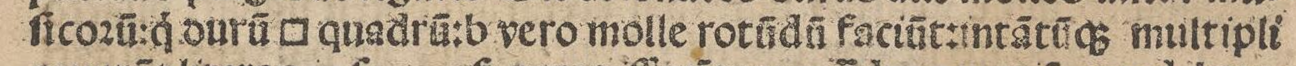
\includegraphics[width=\hsize]{img/149929485-99bdda22-f068-463d-b00d-ac7a9a63a8a2.png}
    \caption{Szarfenberg 1535/1536: astrologiczny znak kwartyl{?}}
    \label{fig:b-durummolleA04}
  \end{figure}
  % https://github.com/psb1558/Junicode-font/discussions/97
  % 'WHITE SQUARE' U+25A1 (Unicode comment: used in astrological contexts for aspect square)
%  Quartile (https://en.wikipedia.org/wiki/Astrological_aspect#Square)

  W edycji Urbańczyka \autocite*[s. 90]{urbańczyk83:_orthog} \textit{b
  durum} oddane jest prawidłowo --- patrz
  il. \vref{fig:b-durummolle-Urb90}.
  Książka ta zawiera również tłumaczenie traktatu przez Józefa
  Dziecha, gdzie występuje ten sam znak
  \autocite*[s. 104]{urbańczyk83:_orthog}--- patrz
  il. \vref{fig:b-durum-Dziech104}.
  

    \begin{figure}[ht]
    \centering
    \includegraphics[height=03ex]{img/00-a_b-durummolle-Urb90}\\
%    \includegraphics[height=03ex]{img/00-b_b-durummolle-Urb90}
    \caption{Edycja Urbańczyka \autocite*{urbańczyk83:_orthog}}
    \label{fig:b-durummolle-Urb90}
  \end{figure}


  
        \begin{figure}[ht]
    \centering
    \includegraphics[height=03ex]{img/00-a_b-durum-Dziech104}%
    \includegraphics[height=03ex]{img/00-b_b-durum-Dziech104}\\
%    \includegraphics[height=03ex]{img/00_b-molle-Dziech104}%
    \caption{Tłumaczenie Dziecha \autocite*{urbańczyk83:_orthog}}
    \label{fig:b-durum-Dziech104}
  \end{figure}

  \subsection{Pierwsze tłumaczenie traktatu (1825)}
\label{sec:pierwsze-tumacz-trak}

  
  Wydawca tłumaczenia traktatu Zaborowskiego przez Kucharskiego
  \autocite*{Kucharski1825} najwyraźniej nie dysponował odpowiednią
  czcionką, znak ten reprezentuje przez ,,czworogran'' słabo
  przypominający oryginał --- patrz
  il. \vref{fig:Kucharsk1825p6Parkosz}.
  
\begin{figure}[t]
    \centering
%    \includegraphics[height=20ex]{img/00_Kucharsk1825p6Parkosz}
    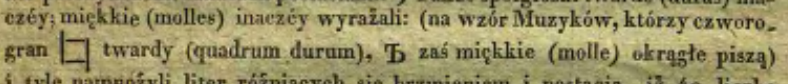
\includegraphics[width=\hsize]{img/KucharskiOCRs6.png}
    \caption{\autocite[s. 6]{Kucharski1825}}
    \label{fig:Kucharsk1825p6Parkosz}
  \end{figure}

  W tłumaczeniu Kucharskiego występuje także \textit{b molle};
  niestety wskutek braku odpowiedniej czcionki ilustracja ta ---
  zawierająca chyba majuskułę twardego znaku
  % (\ucode{042A} \uname{Cyrillic Capital
  %   Letter Hard Sign})
  --- jest myląca, patrz
  il. \vref{fig:Kucharsk1825p6Parkosz}. 

  
\subsection{Pierwsze  wydanie traktatu (1830)}
\label{sec:pierwsze-druk-wydan}

Pierwsze drukowane wydanie to \autocite{samuel30:_jacob_parkos_żoraw}.
Jak widać na il. \vref{fig:b-durum-Bandtkie}, starano się prawidłowo
reprezentować kształt \textit{b durum}, ale związane z tym problemy
techniczne znalazły wyraz w nietrzymaniu linii pisma (chyba czcionkę
odlano niestarannie).


        \begin{figure}[ht]
    \centering
    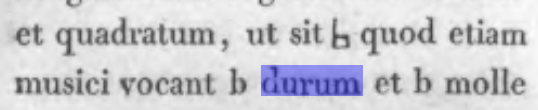
\includegraphics[width=\hsize]{img/BandtkieWBC_OCRlat49bdurum1.png}
    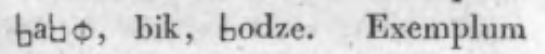
\includegraphics[width=\hsize]{img/BandtkieWBC_OCRlat49bdurum2.png}
    \includegraphics[width=\hsize]{img/Bandtke94alfabet1-1.png}
    \caption{\autocite{samuel30:_jacob_parkos_żoraw} s. 49 i s. 94}
    \label{fig:b-durum-Bandtkie}
  \end{figure}

  Za pomocą specjalnych czcionek starano się możliwie wiernie oddać
  również inne litery Parkosza, tylko \textit{b molle} i \textit{p
    molle} reprezentowano przez zwykłe \textit{b} i \textit{p}.
  
  \subsection{Drugie  wydanie traktatu (1907)}
\label{sec:drug-druk-wydan}

Drugie wydanie traktatu \autocite{Łoś_traktat} oddaje wiernie --- z
jednym niestety wyjątkiem --- wszystkie litery Parkosza, najwyraźniej
został zaprojektowany i wykonany specjalny font. Tym całkowicie
niezrozumiałem wyjątkiem jest \textit{l molle} --- patrz
il. \vref{fig:l-molle-Łoś}.

        \begin{figure}[ht]
    \centering
    \includegraphics[width=\hsize]{img/Łoś37alfabet2-2.png}
    \caption{\autocite{Łoś_traktat} s. 37}
    \label{fig:l-molle-Łoś}
  \end{figure}
  
  Kucała \autocite*[s. 20]{TraktatPWN1985} pisał:
\begin{quote}
  % Trzeba tu zwrócić uwagę, że Parkosz nie stosował w ogóle znaków
  % diakrytycznych. Jedynym wyjątkiem jest \textit{y} z dwiema kropkami
  % (czasem z ukośnymi kreseczkami): \textit{ÿ}, które przejął z pisowni
  % dotychczasowej (podobnie jak \textit{i} z kropką). Nad żadną literą
  % spółgłoskową nie położył ani jednej kreski.
  Na nieporozumieniu
  polega więc twierdzenie, już dawniej spotykane, a ostatnio dość
  stanowczo sformułowane przez S. Jodłowskiego: „Znaki diakrytyczne
  spotykamy m.in. w traktacie [...]  Jakuba Parkoszowica [...] warto
  tu odnotować stosowanie przez Parkoszowica
  % dwu znaków diakrytycznych
  % w postaci dwu poziomo ułożonych kresek nad literą \textit{y} oraz
  [\ldots] przecinka nad literami spółgłoskowymi, mającego zaznaczać
  miękkość spółgłoski"\footnote{\autocite[s. 22-23]{jodłowski79:_losy} --- JSB}.  Nieporozumienie wynikło
  stąd, że J. Łoś w swoim wydaniu traktatu w 1907 r.  zamiast
  \textit{l} z pętelką, jak w rękopisie,
% tzn. I,
  [\ldots]
  dał w transliteracji \textit{l} z przecinkiem u góry [\ldots]
  %: \textit{l'}.
  Za Łosiem to powtarzano, m.in. Z. Klemensiewicz przy omawianiu
  ortografii
  Parkosza\footnote{\autocite[s. 102]{klemensiewicz61:_histor} ---
    JSB}.
  % Parkoszowa ortografia do praktycznego użytku nie była
  % odpowiednia. Nie przyjęto jej więc — nie ma śladów jej stosowania w
  % żadnym XV-wiecznym rękopisie. Ważniejsze znaczenie niż ortograficzne
  % przepisy ma przedstawienie przy okazji formułowania tych przepisów
  % systemu fonologicznego ówczes nej polszczyzny.  1 2 S.  Z.
  % Jodłowski, Losy polskiej ortografii, Warszawa 1979, s. 22-3.
  % Klemensiewicz, Historia języka polskiego, cz. I, Warszawa 1961,
  % s. 102
% [\cite[s. 20]{TraktatPWN1985}]
\end{quote}

\subsection{Trzecie wydanie  i drugie tłumaczenie traktatu (1985)}
\label{sec:wydanie-kucay}
Jak widać, było możliwe stworzenie specjalnego fontu dla wydań z 1830
i 1907 r., jednak było to zapewne zbyt kosztowne lub kłopotliwe w
latach osiemdziesiatych ubiegłego wieku. Dla publikacji
\autocite{TraktatPWN1985} znaki Parkosza zostały narysowane ręcznie
przez grafika, pocięte i wklejone we właściwe miejsca wysiłkiem całego
zespołu redakcyjnego (informacja ustna redaktor książki Zenobii
Mieczkowskiej). Zaletą tego prymitywnego technicznie rozwiązania była
możliwość wiernego oddania kształtów liter, choć nie została ona w
pełni wykorzystana --- il. \vref{fig:bb} pokazuje frament, gdzie dwa
warianty litery \textit{b} sa praktycznie nieodróżnialne; swoją drogą
kształty liter zostały nieznacznie zmodernizowane, bo oryginalne zbyt
odbiegałyby od współczesnych.

        \begin{figure}[ht]
    \centering
    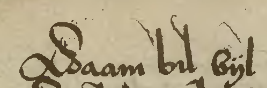
\includegraphics[width=\hsize]{img/ParkoszJBC_Adam.png}
    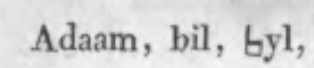
\includegraphics[width=\hsize]{img/BandtkieWBC_OCRlat_Adam.png}
    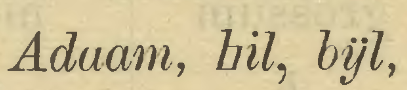
\includegraphics[width=\hsize]{img/Łoś_Adam.png}
    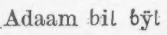
\includegraphics[width=\hsize]{img/Parkosz_55-79_OCRlat_Adam.png}
    \caption{Od góry: rękopis i odczytania Bandtkiego. Łosia i Kucały}
    \label{fig:bb}
  \end{figure}


Litery niewyraźne !!!

\subsection{Wzmianki w druku}
\label{sec:wzmianki-w-druku}

Lisowski w swojej książce \autocite*{lisowski01:_grafia} reprezentuje
\textit{g improprie} przez zwykła literę \textit{q} --- patrz
il. \vref{fig:Lisowski}. Przypuszczam, że inni autorzy też zadowalają
sie przybliżoną reprezentacją znaków Parkosza.

        \begin{figure}[ht]
    \centering
    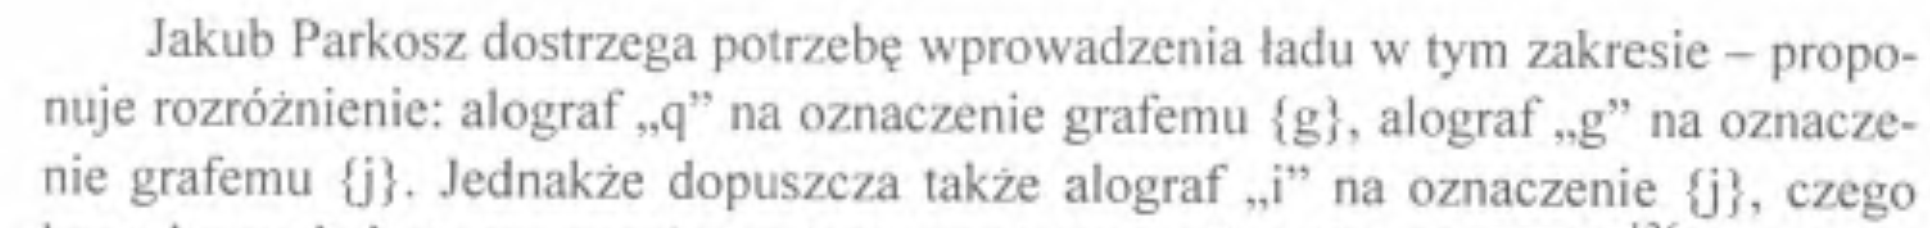
\includegraphics[width=\hsize]{img/GrafiaOCR47g.png}
    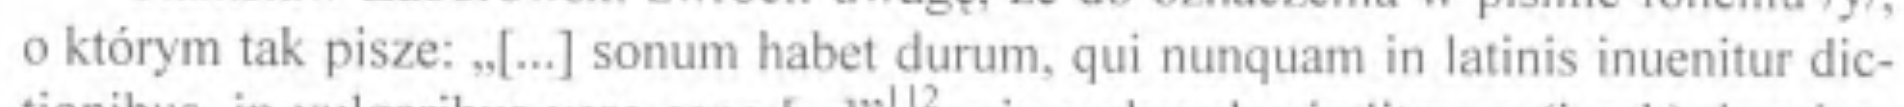
\includegraphics[width=\hsize]{img/GrafiaOCR38q.png}
    \caption{\autocite{lisowski01:_grafia}: litera \textit{q} jako
      \textit{g improprie} (s. 47), niżej przykład litery \textit{q} w
      jej zwykłej funkcji (s. 38)}
    \label{fig:Lisowski}
  \end{figure}


\section{Standard Unicode kodowania znaków}
\label{sec:stand-unic-kodow}

Unicode\footnote{Odmiana tego słowa nie jest ustabilizowana; hasło w
  \textit{Słowniku Gramatycznym Języka Polskiego}
  (\url{http://sgjp.pl/leksemy/\#73537/unicode}) nie reprzentuje
  uzusu, lecz jest tylko propozycją.} to międzynarodowy standard
opracowany i rozwijany przez konsocjum Unicode zrzeszające
m.in. najważniejsze firmy
informatyczne\footnote{\url{https://home.unicode.org}}. Jest on
powszechnie stosowany w komputerach (w tym na stronach WWW),
smartfonach i innym sprzęcie elektronicznym, i nie ma dla niego
alternatywy. Moim zdaniem stanowi on także podstawy współczesnej
grafemiki.

Znak w standardzie Unicode --- \textit{znak kodowy}
(ang. \textit{coded character}) --- to abstrakcyjny obiekt zdefiniowany
przez wyliczenie jego własności z nazwą i przykładowym kształtem
(tzw. glifem) włącznie --- jest to nieco zmieniona i rozbudowana
definicja występująca m.in. w \autocite[s. 11]{bień_stand_unicod1}. W
aktualnej wersji standardu, tj. 15.0.0 z 14 września 2022 r., liczba
znaków wynosi 14\,186. Najważniejszą własnościa znaku jest jego
\textit{punkt kodowy} czyli liczba, która reprezentuje go w
komputerze. Zapisujemy ją w systemie szesnastkowym poprzedzając
prefiksem \texttt{U+}, np. \ucode{018D} (w systemie dziesiątkowym to
liczba 397). Konwencjonalne nazwy znaków są sformułowane w języku
angielskim i zapisywane
wersalikami, % --- w artykule ze względów estetycznych
%stosuję kapitaliki,
np. \uname{LATIN SMALL LETTER TURNED DELTA}. Cytowane glify dla
większej wyrazistości ujmuję w ramki, np.  \gl{ƍ} --- to glif znaku,
którego Grzegorz Seroczyński użył jako Parkoszowego \textit{g
  improprie} w swoich omówieniach traktatu \autocite*{Serocz17},
\autocite* {Serocz14}. Z własnościami tego i innych znaków można
zapoznać się m.in. pod adresem
\url{https://util.unicode.org/UnicodeJsps/properties.html},
por. il. \vref{fig:properties}.

        \begin{figure}[ht]
    \centering
    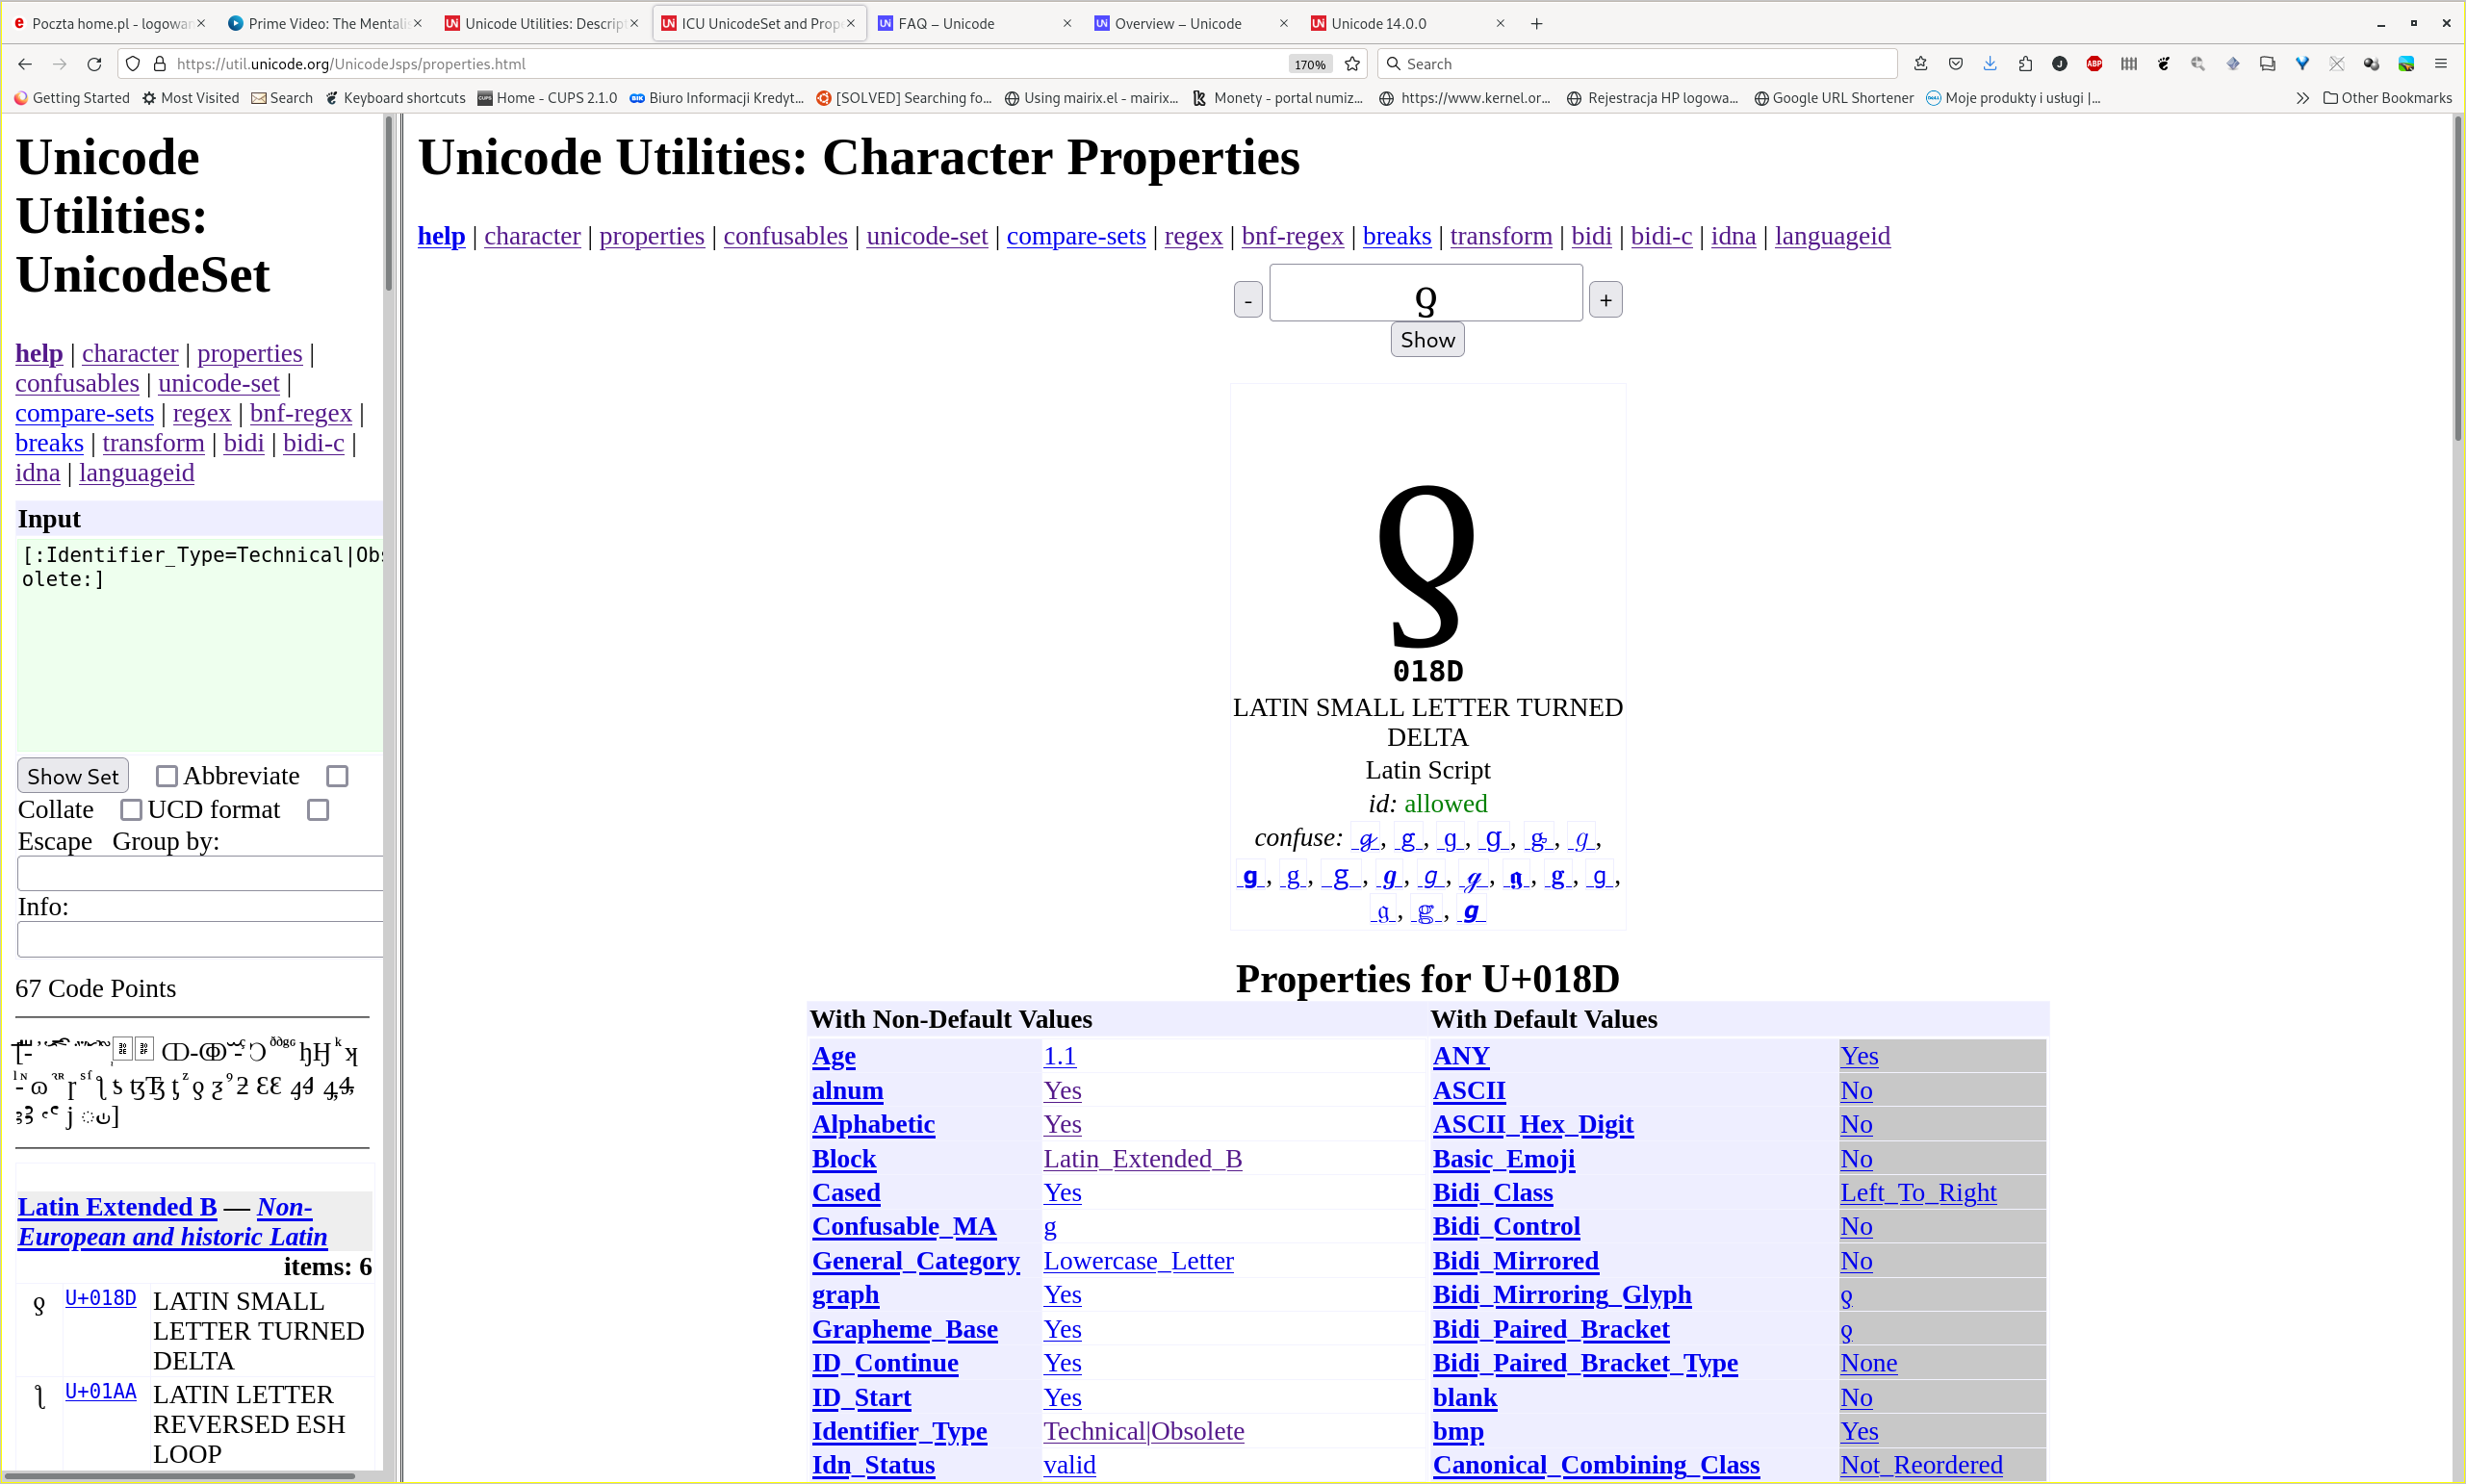
\includegraphics[width=\hsize]{img/U+018D.png}
    \caption{Własności znaku \gl{ƍ} \ucode{018D} \uname{LATIN SMALL
        LETTER TURNED DELTA} --- jest ich ponad 160}
    \label{fig:properties}
  \end{figure}

  W standardzie występuje pojęcie \textit{znaku obserwowanego} (to
  moje swobodne tłumaczenie ang. \textit{user-perceived
    character}). Taki obiekt wolę nazywać \textit{tekstelem}
  (elementem tekstu). Tekstel może być reprezentowany przez pojedynczy
  znak kodowy (,,singleton'') lub przez sekwencję znaków kodowych
  (pierwszy znak nazywa się znakiem bazowym); niektóre tekstele mogą
  być reprezentowane na kilka sposobów. Najważniejsze sekwencje znaków
  są trojakiego rodzaju:
  \begin{itemize}
  \item znak bazowy i znaki dostawne (ang. \textit{combining characters)},
  \item znak bazowy i selektor wariantu (ang. \textit{variation selector}),
  \item znak bazowy i znak lub znaki etykietowe (ang. \textit{tag characters}).
  \end{itemize}

  % https://en.wikipedia.org/wiki/Miscellaneous_Symbols_and_Pictographs#Emoji_modifiers
  % https://pl.wikipedia.org/wiki/Fototypy_sk%C3%B3ry
  
  Przykładem tekstela reprezentowanego przez singleton jest \gl{ć}
  \ucode{0107} \uname{LATIN SMALL LETTER C WITH ACUTE}. Tekstel ten
  może też być reprezentowany przez sekwencję: znak bazowy \gl{c}
  \ucode{0063} \uname{LATIN SMALL LETTER C} i znak dostawny \gl{◌́}
  (oczywiście kółko nie jest częścią glifu, lecz służy do pokazania pozycji znaku
  dostawnego względem znaku bazowego) \ucode{0301} \uname{COMBINING
    ACUTE ACCENT}; sekwencję taką zapisujemy
  <\ucode{0063},\ucode{0301}>.

% https://unicode.org/Public/UCD/latest/ucd/StandardizedVariants.txt  
  Drugi typ sekwencji z użyciem selectora wariantu jest stosowany
  przede wszystkim dla sinogramów, inne zastosowania --- znaki
  matematyczne, język mongolski, język birmański
  (ang. \textit{Myanmar}), tybetańskie pismo phags-pa, pismo
  manichejskie (ang. \textit{Manichaean}) i hieroglify egipskie --- są
  z naszej perspektywy też mało interesujące.
% 15.0: Egyptian hieroglyph rotational variants

  Trzeci typ sekwencji był dotąd stosowany w praktyce wyłącznie do
  znaków bazowych, które nazywam nie w pełni precyzyjnie
  piktogramami\footnote{Chodzi konkretnie o \textit{emoji},
    por. np. \url{https://pl.wikipedia.org/wiki/Emoji}. Dla pełności
    obrazu można dodać, ze czwarty typ sekwencji stosuje sie tylko do
    \textit{emoji} oznaczających ludzi i części ciała, a specjalny
    modyfikator oznacza fototyp skóry według klasyfikacji
    Fitzpatricka.}
  % https://pl.wikipedia.org/wiki/Fototypy_sk%C3%B3ry
  % https://en.wikipedia.org/wiki/Miscellaneous_Symbols_and_Pictographs
; nie ma jednak żadnego technicznego ani formalnego
  ograniczenia ich użycia --- w szczególności w przeciwieństwie do
  selektorów wariantu użycia te nie muszą być zatwierdzane przez
  konsorcjum Unicode. Przykładem może być flaga Szkocji, którą
  reprezentujemy jako sekwencję \uname{BLACK FLAG}, 󠁧 \uname{TAG LATIN
    SMALL LETTER G}, 󠁢 \uname{TAG LATIN SMALL LETTER B}, 󠁳 \uname{TAG
    LATIN SMALL LETTER S}, 󠁣 \uname{TAG LATIN SMALL LETTER C}, 󠁴
  \uname{TAG LATIN SMALL LETTER T}, 󠁿 \uname{CANCEL TAG}\footnote{Patrz
    np.. \url{https://emojipedia.org/flag-scotland/}.}. Znaki
  etykietowe są w zasadzie niewidzialne, ale na potrzeby dyskusji i
  dokumentacji mogą być wizualizowane, np. \ucode{E0070} \uname{TAG
    LATIN SMALL LETTER P} może być prezentowany jako {\Ji{\&\_\_p;}}.


  Na potrzeby elektronicznej edycji traktatu Parkosza w odczytaniu
  Kucały \autocite*{kucała20:_trakt_jakub_parkos} został opracowany
  system transliteracji wykorzystujący wyłącznie znaki kodowe mające
  formalnie własność litery. Założenia tej transliteracji zostały
  przedstawione w artykule \autocite{bien_parkoszPSP}. 
% na
%  \vref{kropki}.
% !!!

  Ponieważ transliteracja zmienia oryginalne znaczenie znaków,
  potrzebna jest metainformacja pozwalajaca odróżnić transliterację od
  normalnego tekstu. Można tego uniknąć wprowadzająć dodatkowe znaki
  jako tzw. znaki prywatne. Dobrym przykładem wykorzystania w
  standardzie Unicode znaków prywatnych jest Medieval Unicode Font
  Initiative\footnote{\url{https://mufi.info}} (dalej MUFI). Znaki
  prywatne maja swoje punkty kodowe i nazwy, w zapisie punktów
  kodowych proponuję używać prefiksu \texttt{M+} zamiast \texttt{U+};
  znaki prywatne sa całkowicie pozbawione własności, co może utrudniać
  przetwarzanie. Przykładem znaków prywatnych mogą być \gl{}
  \mcode{F223} \uname{LATIN SMALL LETTER M WITH RIGHT DESCENDER} i
  \gl{} \mcode{F228} \uname{LATIN SMALL LETTER N WITH RIGHT
    DESCENDER}; o znakach tych będziemy jeszcze mówić w dalszym ciągu
  artykułu.

  Możliwe jest również inne wygodniejsze rozwiązanie, które zostało
  przedstawione w artykule \autocite{bien_representing_2022} i
  zostanie w skrócie omówione dalej. Tak czy inaczej niezbędny jest
  odpowiedni font.
  


\section{Font Junicode}
\label{sec:font-junicode}

Font Junicode stworzył i od ponad 20 lat rozwija hobbystycznie Peter S. Baker
\autocite*{baker22:Junicode}, profesor angielskiej literatury
średniowiecznej na Uniwersytecie Wirginii. Nazwa fontu, będąca skrótem
od \textit{Junius
  Junicode}\footnote{\url{https://en.wikipedia.org/wiki/Junicode}},
miała być prowizoryczna, ale próba jej zmiany na JuniusX wywołała
tylko zamieszanie. Font jest udostępniony na otwartej licencji: każdy
może go nie tylko rozpowszechniać, ale również modyfikować i
rozpowszechniać wersję zmodyfikowaną.

Font jest przeznaczony dla mediewistów, co przejawia się m.in. we
włączeniu do repertuaru wszystkich znaków prywatnych z rekomendacji
MUFI (najnowsze dodatki do rekomendacji dostępne są tylko w
wyszukiwarce na witrynie MUFI, do wersji 4 rekomendacje miały formę
dokumentów PDF).

Dla polskiego użytkownika font Junicode był interesujący już wcześniej z powodu
uwzględnienia znaków niezbędnych do cytowania m.in. traktatu Zaborowskiego
(\autocite{bień21:_usage_unicod_plane_junius_polis},
  \autocite{bień22:trakt_stanis_zabor_A}). 

Na uwagę zasługuje intensywne wykorzystywanie tzw. funkcji zecerskich
(ang. \textit{typographical features}) dostępnych w zastosowanych
formatach TrueType i OpenType; zalety tego podejścia są przedstawione
w cytowanej już dokumentacji \autocite{baker22:Junicode}.

W marcu 2022 r, Margaret Kibi (\texttt{marrus-sh}) zaproponowała
stosowanie znaków etykietowych w charakterze prywatnych selektorów
wariantów\footnote{\raggedright
  \url{github.com/psb1558/Junicode-font/discussions/122\#discussioncomment-2416880}}.
Ta idea została wykorzystana m.in. do znaków Parkosza.  Obecnie w
wersjach fontu Junicode z 25 sierpnia 2022 r. i późniejszych dostępne
są m.in. znaki przedstawione na il. \vref{fig:Parkosz}.


Znaki te są dostępne po wybraniu funkcji zecerskiej \textit{Stylistic
  Set 10}. Na końcowym etapie opracowania niniejszy artykuł był
edytowany w angielskojęzycznej wersji programu LibreOffice, gdzie w
tym celu najpierw został zaznaczony odpowiedni fragment tekstu,
następnie z menu ``Format'' została wybrana pozycja ``Character''; po
wybraniu fontu został użyty przycisk ``Feature'', gdzie dokonano
wyboru ``Stylisti Set 10'' --- patrz il. \vref{fig:OOCharacter} i
\vref{fig:OOFont}. Ponieważ nie jestem regularnym użytkownikiem tego
programu, nie mogę zagwarantować, że ta procedura jest optymalna.

        \begin{figure}[ht]
    \centering
    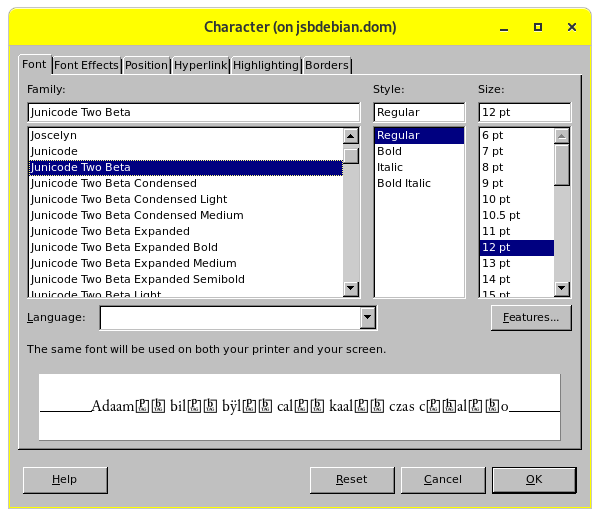
\includegraphics[width=\hsize]{img/OO_Character.png}
    \caption{LibreOffice: wybór fontu}
    \label{fig:OOCharacter}
  \end{figure}

        \begin{figure}[ht]
    \centering
    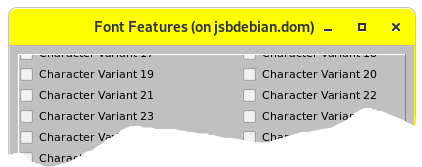
\includegraphics[width=\hsize]{img/OO_FontFeatures1.png}
    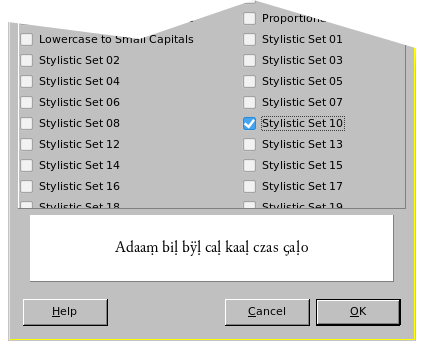
\includegraphics[width=\hsize]{img/OO_FontFeatures2.png}
    \caption{LibreOffice: wybór funkcji zecerskiej}
    \label{fig:OOFont}
  \end{figure}



Do znaku
bazowego dodawane sa dwa znaki etykietowe, które w języku angielskim
mają znaczenie mnemotechniczne: pierwszy znak to {\Ji{\&\_\_p;}}
oznaczający znaki Parkosza. Drugie w kolejności znaki etykietowe to
{\Ji{\&\_\_s;}} \textit{square} (\textit{kwadratowy}), \Ji{\&\_\_r;}
\textit{round} (\textit{okragły)}, \Ji{\&\_\_h;} \textit{hook}
(\textit{haczyk}), \Ji{\&\_\_l;} \textit{loop} (\textit{pętla}),
\Ji{\&\_\_s;} \textit{slashed} (\textit{przekreślony}), \Ji{\&\_\_b;}
\textit{below} (\textit{poniżej}), \Ji{\&\_\_d;} \textit{descender}
(\textit{wydłużenie dolne}) lub \textit{dot} (\textit{kropka}).


        \begin{figure}[ht]
    \centering
{\relsize{5}
  {\gl{b\&\_\_p;\&\_\_s;}}
  {\gli{b\&\_\_p;\&\_\_s;}}
  {\glb{b\&\_\_p;\&\_\_s;}}
  {\gl{b\&\_\_p;\&\_\_l;}}
  {\gli{b\&\_\_p;\&\_\_l;}}
  {\glb{b\&\_\_p;\&\_\_l;}}
  {\gl{p\&\_\_p;\&\_\_s;}}
  {\gli{p\&\_\_p;\&\_\_s;}}
  {\glb{p\&\_\_p;\&\_\_s;}}
  {\gl{p\&\_\_p;\&\_\_r;}}
  {\gli{p\&\_\_p;\&\_\_r;}}
  {\glb{p\&\_\_p;\&\_\_r;}}

  {\gl{l\&\_\_p;\&\_\_l;}}
  {\gli{l\&\_\_p;\&\_\_l;}}
  {\glb{l\&\_\_p;\&\_\_l;}}
  {\gl{v\&\_\_p;\&\_\_h;}}
  {\gli{v\&\_\_p;\&\_\_h;}}
  {\glb{v\&\_\_p;\&\_\_h;}}
  {\gl{g\&\_\_p;\&\_\_h;}}
  {\gli{g\&\_\_p;\&\_\_h;}}
  {\glb{g\&\_\_p;\&\_\_h;}}
  {\gl{c\&\_\_p;\&\_\_h;}}
  {\gli{c\&\_\_p;\&\_\_h;}}
  {\glb{c\&\_\_p;\&\_\_h;}}

  {\gl{P\&\_\_p;\&\_\_s;}}
  {\gli{P\&\_\_p;\&\_\_s;}}
  {\glb{P\&\_\_p;\&\_\_s;}}
  {\gl{P\&\_\_p;\&\_\_r;}}
  {\gli{P\&\_\_p;\&\_\_r;}}
  {\glb{P\&\_\_p;\&\_\_r;}}
}
\caption{\textit{b grossum}, \textit{b molle}, \textit{p durum},
  \textit{p molle}, \textit{l molle}, \textit{durum v}, \textit{g
    improprie}, nienazwany wariant litery \textit{c}, majuskuły:
  \textit{p grossum}, \textit{p molle}}
    \label{fig:Parkosz}
  \end{figure}

  Mamy więc {\Ji{b\&\_\_p;\&\_\_s;}} ({\gl{b\&\_\_p;\&\_\_s;}}),
  {\Ji{b\&\_\_p;\&\_\_l;}} ({\gl{b\&\_\_p;\&\_\_l;}}),
  {\Ji{p\&\_\_p;\&\_\_s;}} ({\gl{p\&\_\_p;\&\_\_s;}}),
  {\Ji{p\&\_\_p;\&\_\_r;}} ({\gl{p\&\_\_p;\&\_\_r;}}),
  {\Ji{l\&\_\_p;\&\_\_l;}} ({\gl{l\&\_\_p;\&\_\_l;}}),
  {\Ji{v\&\_\_p;\&\_\_h;}} ({\gl{v\&\_\_p;\&\_\_h;}}),
  {\Ji{g\&\_\_p;\&\_\_h;}} ({\gl{g\&\_\_p;\&\_\_h;}}),
  {\Ji{c\&\_\_p;\&\_\_h;}} ({\gl{c\&\_\_p;\&\_\_h;}}),
  {\Ji{P\&\_\_p;\&\_\_s;}} ({\gl{P\&\_\_p;\&\_\_s;}}),
  {\Ji{P\&\_\_p;\&\_\_r;}} ({\gl{P\&\_\_p;\&\_\_r;}}).
  
  Jak wiadomo, traktat Parkosza zachował się w kopii, w dodatku
  pisanej przez dwóch skrybów, w konsekwencji nie wiadomo, w jakim
  stopniu kształt liter rękopisu oddaje intencje Parkosza. Dotyczy to
  przede wszystkim \textit{grossum m} i \textit{grossum n}.  Z jednej
  strony Parkosz pisze, ze kształt litery jest taki, jak na końcu
  słowa --- przynajmniej w części Europy wyglądał on tak, jak na na
  il. \vref{fig:ParkoszMN}, co potwierdza
  np. \autocite{emiliano:_the_portug_mediev_font_projec}. Z drugiej
  strony Parkosz pisze, że należy pisać te litery z \textit{cauda}
  czyli ogonkiem. Łoś i Kuczała interpretują ogonek jako wydłużenie
  dolne wygięte w prawo, natomiast w rękopisie ostatnia kreska
  (,,minim'') litery jest po prostu wydłużona i ten kształt zachował
  Bandtkie --- patrz \autocite[s.41]{bień22:_parkosT} (il. 8).
  
        \begin{figure}[ht]
    \centering
{\relsize{5}
  \gl{m\&\_\_p;\&\_\_d;}
  \gli{m\&\_\_p;\&\_\_d;}
  \glb{m\&\_\_p;\&\_\_d;}
  \gl{n\&\_\_p;\&\_\_d;}
  \gli{n\&\_\_p;\&\_\_d;}
  \glb{n\&\_\_p;\&\_\_d;}

  }
    \caption{\textit{grossum m}? \textit{grossum n}?}
    \label{fig:ParkoszMN}
  \end{figure}

  Peter Baker zaproponował, żeby \textit{grossum m}
  ({\Ji{m\&\_\_p;\&\_\_d;}}) i \textit{grossum n}
  ({\Ji{n\&\_\_p;\&\_\_d;}}) reprezentować przez wspomniane wcześniej
  znaki \mcode{F223} \uname{LATIN SMALL LETTER M WITH RIGHT DESCENDER}
  i \mcode{F228} \uname{LATIN SMALL LETTER N WITH RIGHT DESCENDER},
  przedstawione na il. \vref{fig:ParkoszMN}. Decyzję te
  zaakceptowałem, choc nie traktuję jej jako ostateczną. Jeśli ktoś się
  z tą decyzją nie zgadza, może na witrynie repozytorium
  fontu\footnote{\url{https://github.com/psb1558/Junicode-font}}
  otworzyć dyskusję lub zgłosić konkretny postulat.

  W transliteracji traktatu \autocite{kucała20:_trakt_jakub_parkos}
  nowatorską (ale kontrowersyjną) decyzją było dodanie kropek do liter
  o standardowym kształcie, ale innej niż współczesna wartości
  fonetycznej. Aby ułatwić chętnym stosowanie tej konwencji litery te
  mogą być wprowadzane za pomocą znaków etykietowych, np. \ucode{1E1F}
  \uname{LATIN SMALL LETTER F WITH DOT ABOVE} (\gl{ḟ})jako
  {\Ji{f\&\_\_p;\&\_\_d;}}. Pełny wykaz takich ułatwień znajduje się w
  dokumentacji fontu i artykule \autocite{bien_representing_2022}.

  Font Junicode został wykorzystany do przygotowania wstępnej wersji
  nowej edycji elektronicznej traktatu, dostępnej w repozytorium
  Zenodo\footnote{\url{https://doi.org/10.5281/zenodo.3883862}} i w
  formie źródłowej w
  repozytorium\footnote{\url{https://github.com/jsbien/Parkosz-traktat/}},
  por. il. \vref{fig:edycja}.

        \begin{figure}[ht]
    \centering
    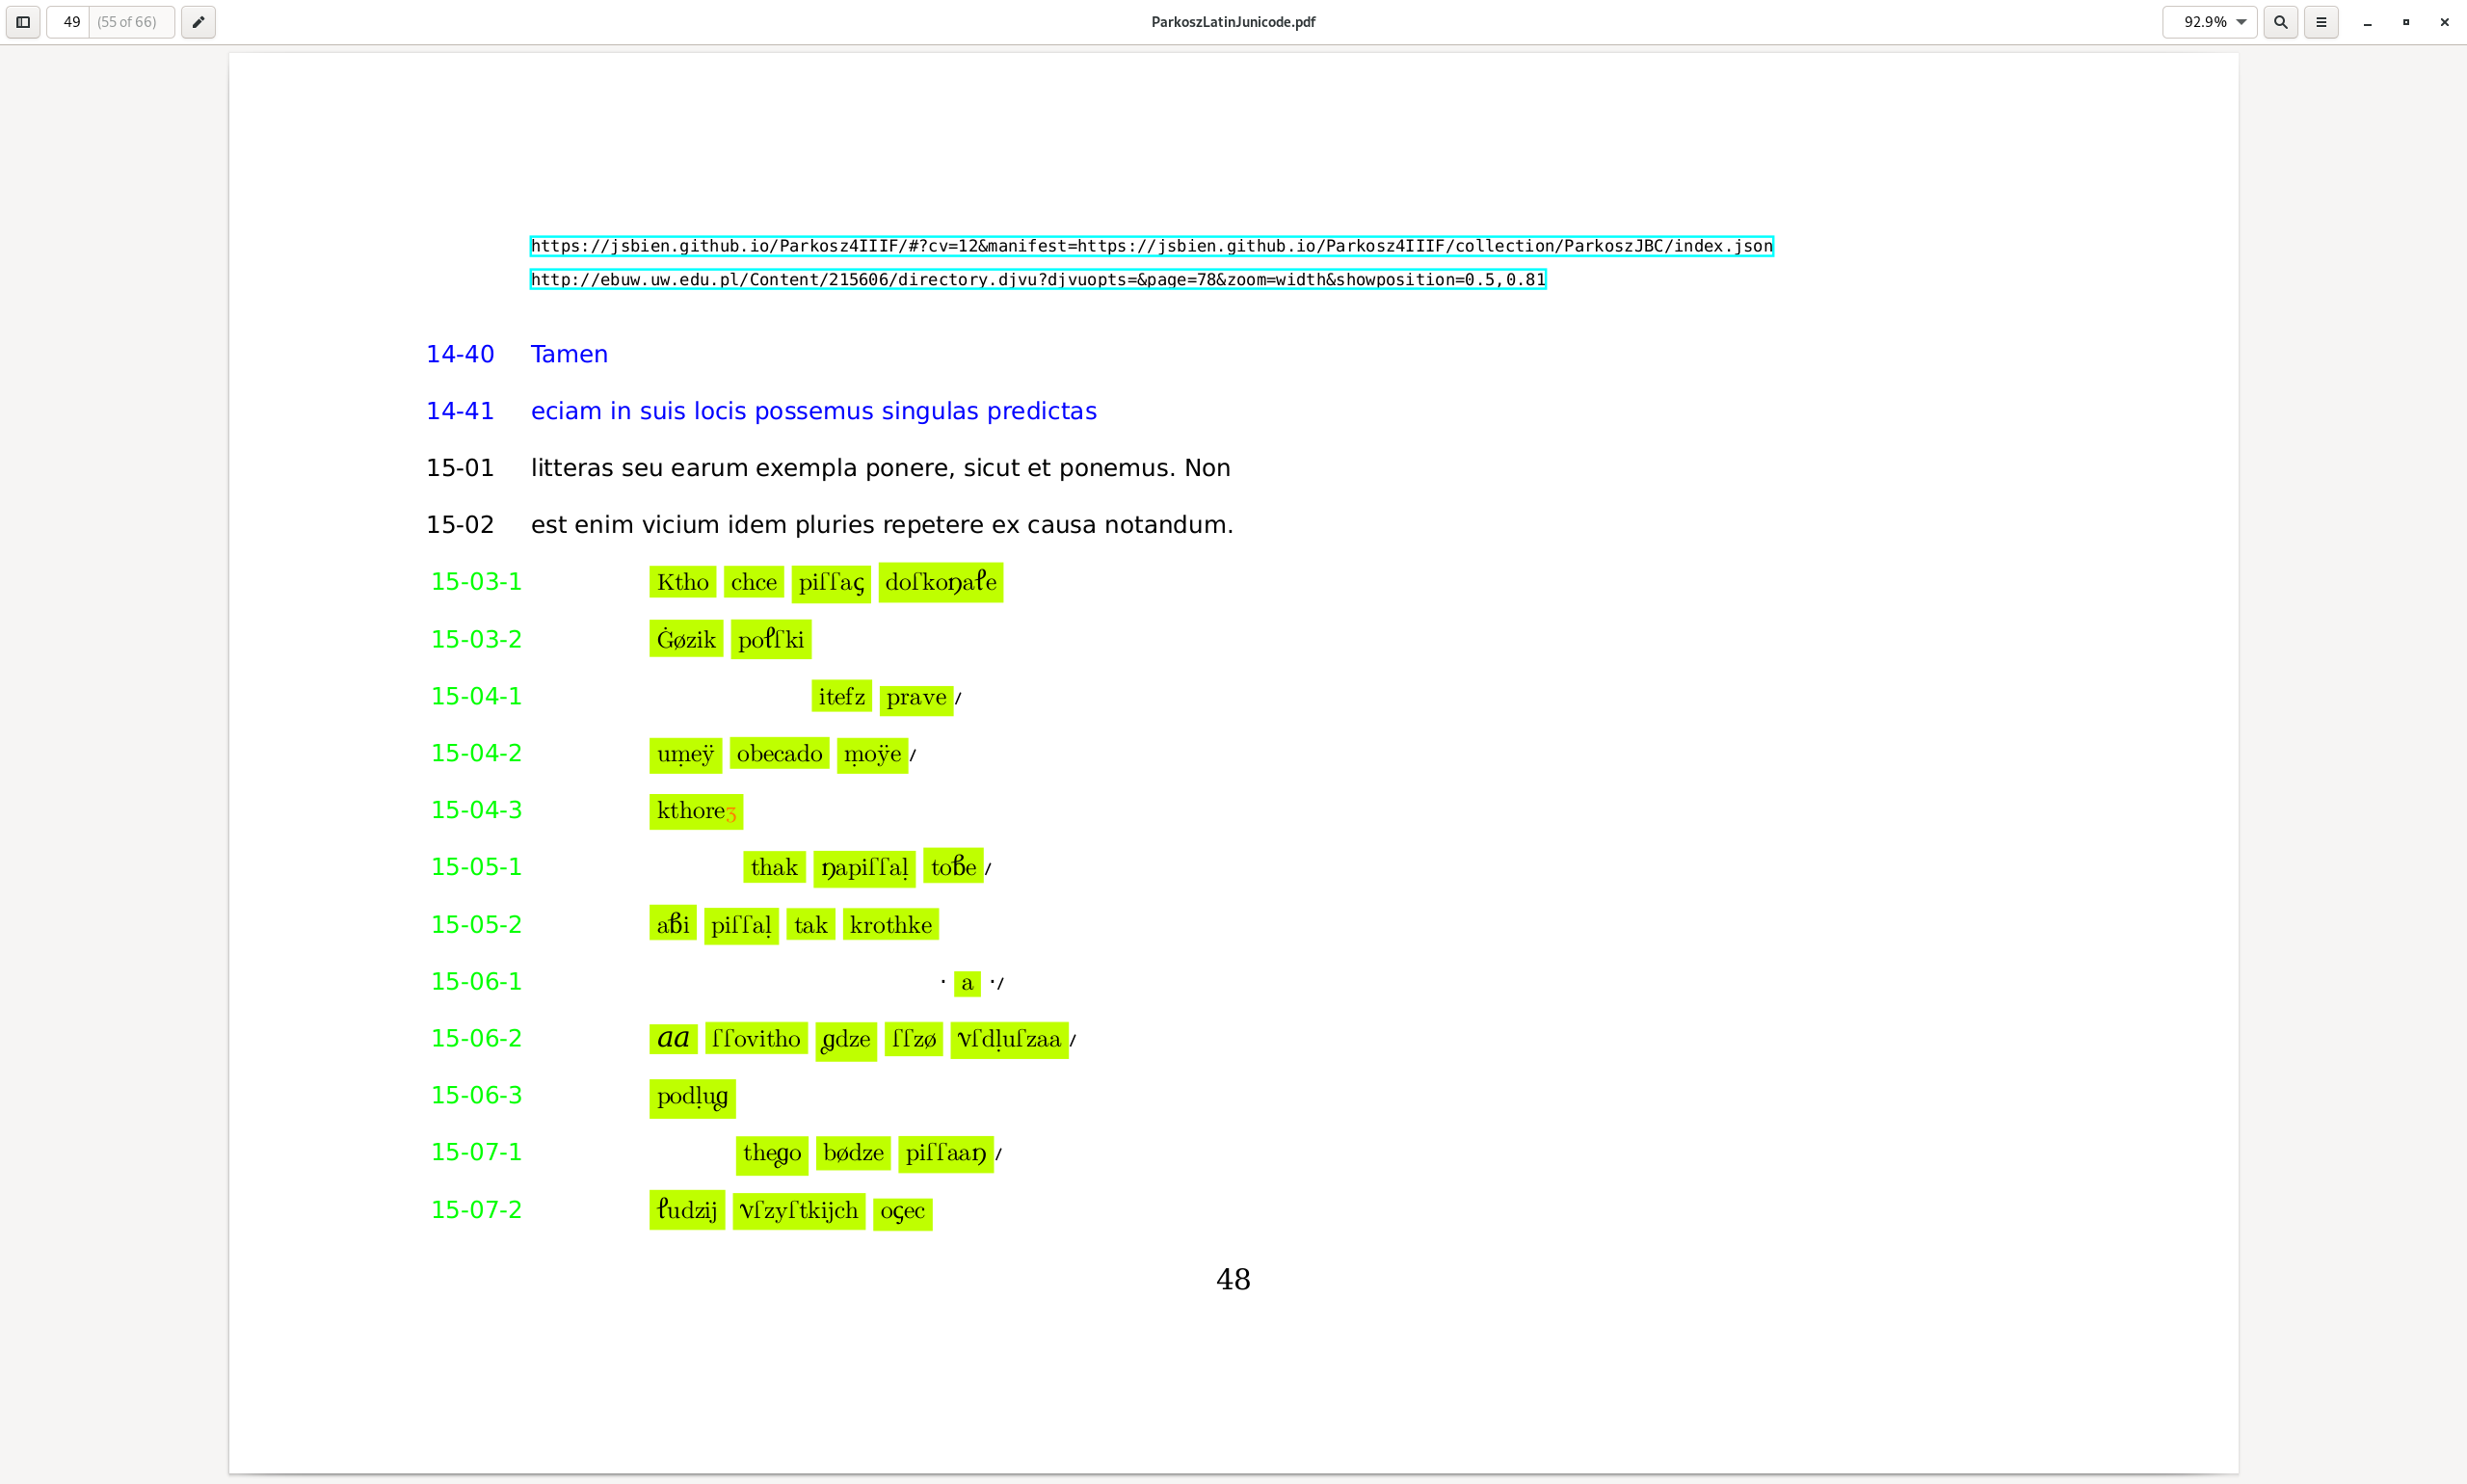
\includegraphics[width=\hsize]{img/edycja.png}
    \caption{Fragment nowej elektronicznej edycji traktatu 
      (logiczny podział na wiersze jest uzupełniony na lewym marginesie
      o informację o podziale oryginalnym)}
    \label{fig:edycja}
  \end{figure}

  
  Lista polskich słów znajdująca się pod koniec traktatu w foncie
  Junicode może więc prezentować się następująco:
  \label{kropki}



  \begin{quote}\raggedright
%Adaaṃ
Adaa\sgl{m\&\_\_p;\&\_\_b;}    
%biḷ
%bi{\sgl{l\&\_\_p;\&\_\_b;}}
{\sgl{b\&\_\_p;\&\_\_s;}}i{\sgl{l\&\_\_p;\&\_\_b;}}
%bÿḷ
%bÿ{\sgl{l\&\_\_p;\&\_\_b;}}
{\sgl{b\&\_\_p;\&\_\_l;}}ÿ{\sgl{l\&\_\_p;\&\_\_b;}}
%caḷ
ca{\sgl{l\&\_\_p;\&\_\_b;}}
%kaal
kaa{\sgl{l\&\_\_p;\&\_\_b;}}
%czas
czas
%çaḷo
\sgl{c\&\_\_p;\&\_\_h;}a{\sgl{l\&\_\_p;\&\_\_b;}}o
%chood
chood
%daaḷ
daa{\sgl{l\&\_\_p;\&\_\_b;}}
%dzaaḷ
dzaa{\sgl{l\&\_\_p;\&\_\_b;}}
%eſz
e\sgl{s\&\_\_l;\&\_\_o;}z
%ffitaa
ffitaa
%fiꝿi
fi\sgl{g\&\_\_p;\&\_\_h;}i
i
%ġee
\sgl{{g\&\_\_p;\&\_\_d;}}ee
%ÿe
ÿe
%ꝿhaaɲ
\sgl{g\&\_\_p;\&\_\_h;}haa\sgl{n\&\_\_d;\&\_\_c;}
%kroɬ
kro{\sgl{l\&\_\_p;\&\_\_l;}}
%ḷis
{\sgl{l\&\_\_p;\&\_\_b;}}is
%ɬis
{\sgl{l\&\_\_p;\&\_\_l;}}is
%ɱikaa
{\sgl{m\&\_\_p;\&\_\_d;}}ikaa
% ṃika
{\sgl{m\&\_\_p;\&\_\_b;}}ika
%ɲiſſki
{\sgl{n\&\_\_p;\&\_\_d;}}iſſki
%ṇiſki
{\sgl{n\&\_\_p;\&\_\_b;}}iſki
%othooſz
othooſz
%ƥiġe
{\sgl{p\&\_\_p;\&\_\_r;}}i\sgl{{g\&\_\_p;\&\_\_d;}}e
%piſchṇo literówka u Kucały
{\sgl{p\&\_\_p;\&\_\_r;}}iſchno
%qʋras
q{\sgl{v\&\_\_p;\&\_\_h;}}ras
%roſſa
roſſa
%rzøøſſa
rzøøſſa
%roſuuɱ.
roſuu{\sgl{m\&\_\_p;\&\_\_d;}}
%ſaaɱ
ſaa{\sgl{m\&\_\_p;\&\_\_b;}}
%ſchaad
ſchaad
%ſſzaadḷ
ſſzaad{\sgl{l\&\_\_p;\&\_\_b;}}
%ſzak 
ſzak 
%zzaraa
zzaraa
%Zaɱɲø
Za{\sgl{m\&\_\_p;\&\_\_d;}}{\sgl{n\&\_\_p;\&\_\_d;}}ø
%to
to
%uṃee
u{\sgl{m\&\_\_p;\&\_\_b;}}ee
%uuɲ
uu{\sgl{n\&\_\_p;\&\_\_d;}}
%viḷa
vi{\sgl{l\&\_\_p;\&\_\_b;}}a
%ʋiɬaaḷ
ʋi{\sgl{l\&\_\_p;\&\_\_l;}}aa{\sgl{l\&\_\_p;\&\_\_b;}}
%wſta
wſta
%xøøodz
xøøodz
%ÿⱥṇczøc
ÿⱥnczøc
%ÿoczi
ÿoczi
%ÿøøkaa
ÿøøkaa

  \end{quote}

% Tags for Jakub Parkosz, Traktat o ortografii Polskiej
%Parkosz_tags.pdf

%  https://github.com/psb1558/Junicode-font/discussions/97

\section{Uwagi końcowe}
\label{sec:uwagi-kocowe}

Wprowadzanie znaków etykietowych można sobie ułatwiać na różne
sposoby, tutaj wspomnimy tylko o jednej, specyficznej dla fontu
Junicode. Znak \ucode{E0070} \uname{TAG LATIN SMALL LETTER P}
({\Ji{\&\_\_p;}}) może być wprowadzony sekwencją \verb|\&\_\_p;|, znak
\ucode{E0073} \uname{TAG LATIN SMALL LETTER S} ({\Ji{\&\_\_p;}}) może
być wprowadzony sekwencją {\verb|\&\_\_s;|} itp. --- nie wymaga to
pamiętania punktów kodowych, a dodatkowo sekwencję taka można
przypisać jakiemuś skrótowi klawiaturowemu.

Bezpośrednie użycie fontu Junicode na stronach internetowej nie jest
wskazane, ponieważ ci użytkownicy, którzy nie mają na swoim komputerze
zainstalowanego tego fontu, zamiast specyficznych dla fontu znaków
zobaczą czarne prostokąty (tzw. tofu). Problem jest ogólny i znany od
dawna, jego rozwiązaniem jest tzw. \textit{ Web Open Font Format}
(aktualnie w wersji 2, w skrócie WOFF2). Fonty w tym formacie mogą być umieszczone na
stronie internetowej i pobrane automatycznie przez przeglądarkę.

Aby nie spowalniać ładowania strony, bardzo wskazane jest stworzenie
\textit{ad hoc} fontu zawierającego tylko znaki występujące na danej
stronie. Jeśli na stronie font jest używany w kilku odmianach
(np. antykwa i kursywa), to warto użyć tzw. fontu zmiennego
(ang. \textit{variable font}).

W dokumentacji \autocite{baker22:Junicode} można znaleźć pożyteczne
informacje na temat zmiennego wariantu fontu Junicode oraz narzędzi do
konwersji na podzbiór fontu w w formacie WOFF2.



%https://github.com/psb1558/Junicode-font/discussions/146#discussioncomment-3544745



\printbibliography

\end{document}


%%% Local Variables:
%%% mode: latex
%%% ispell-local-dictionary: "polish"
%%% TeX-master: "JSB_Parkosz_font"
%%% coding: utf-8-unix
%%% TeX-PDF-mode: t
%%% TeX-engine: xetex
%%% End:
